% =================
% Sector Shangra Omega
% =================

\section{Sector Shangra Omega}
\label{sec:sector}

\begin{center}
  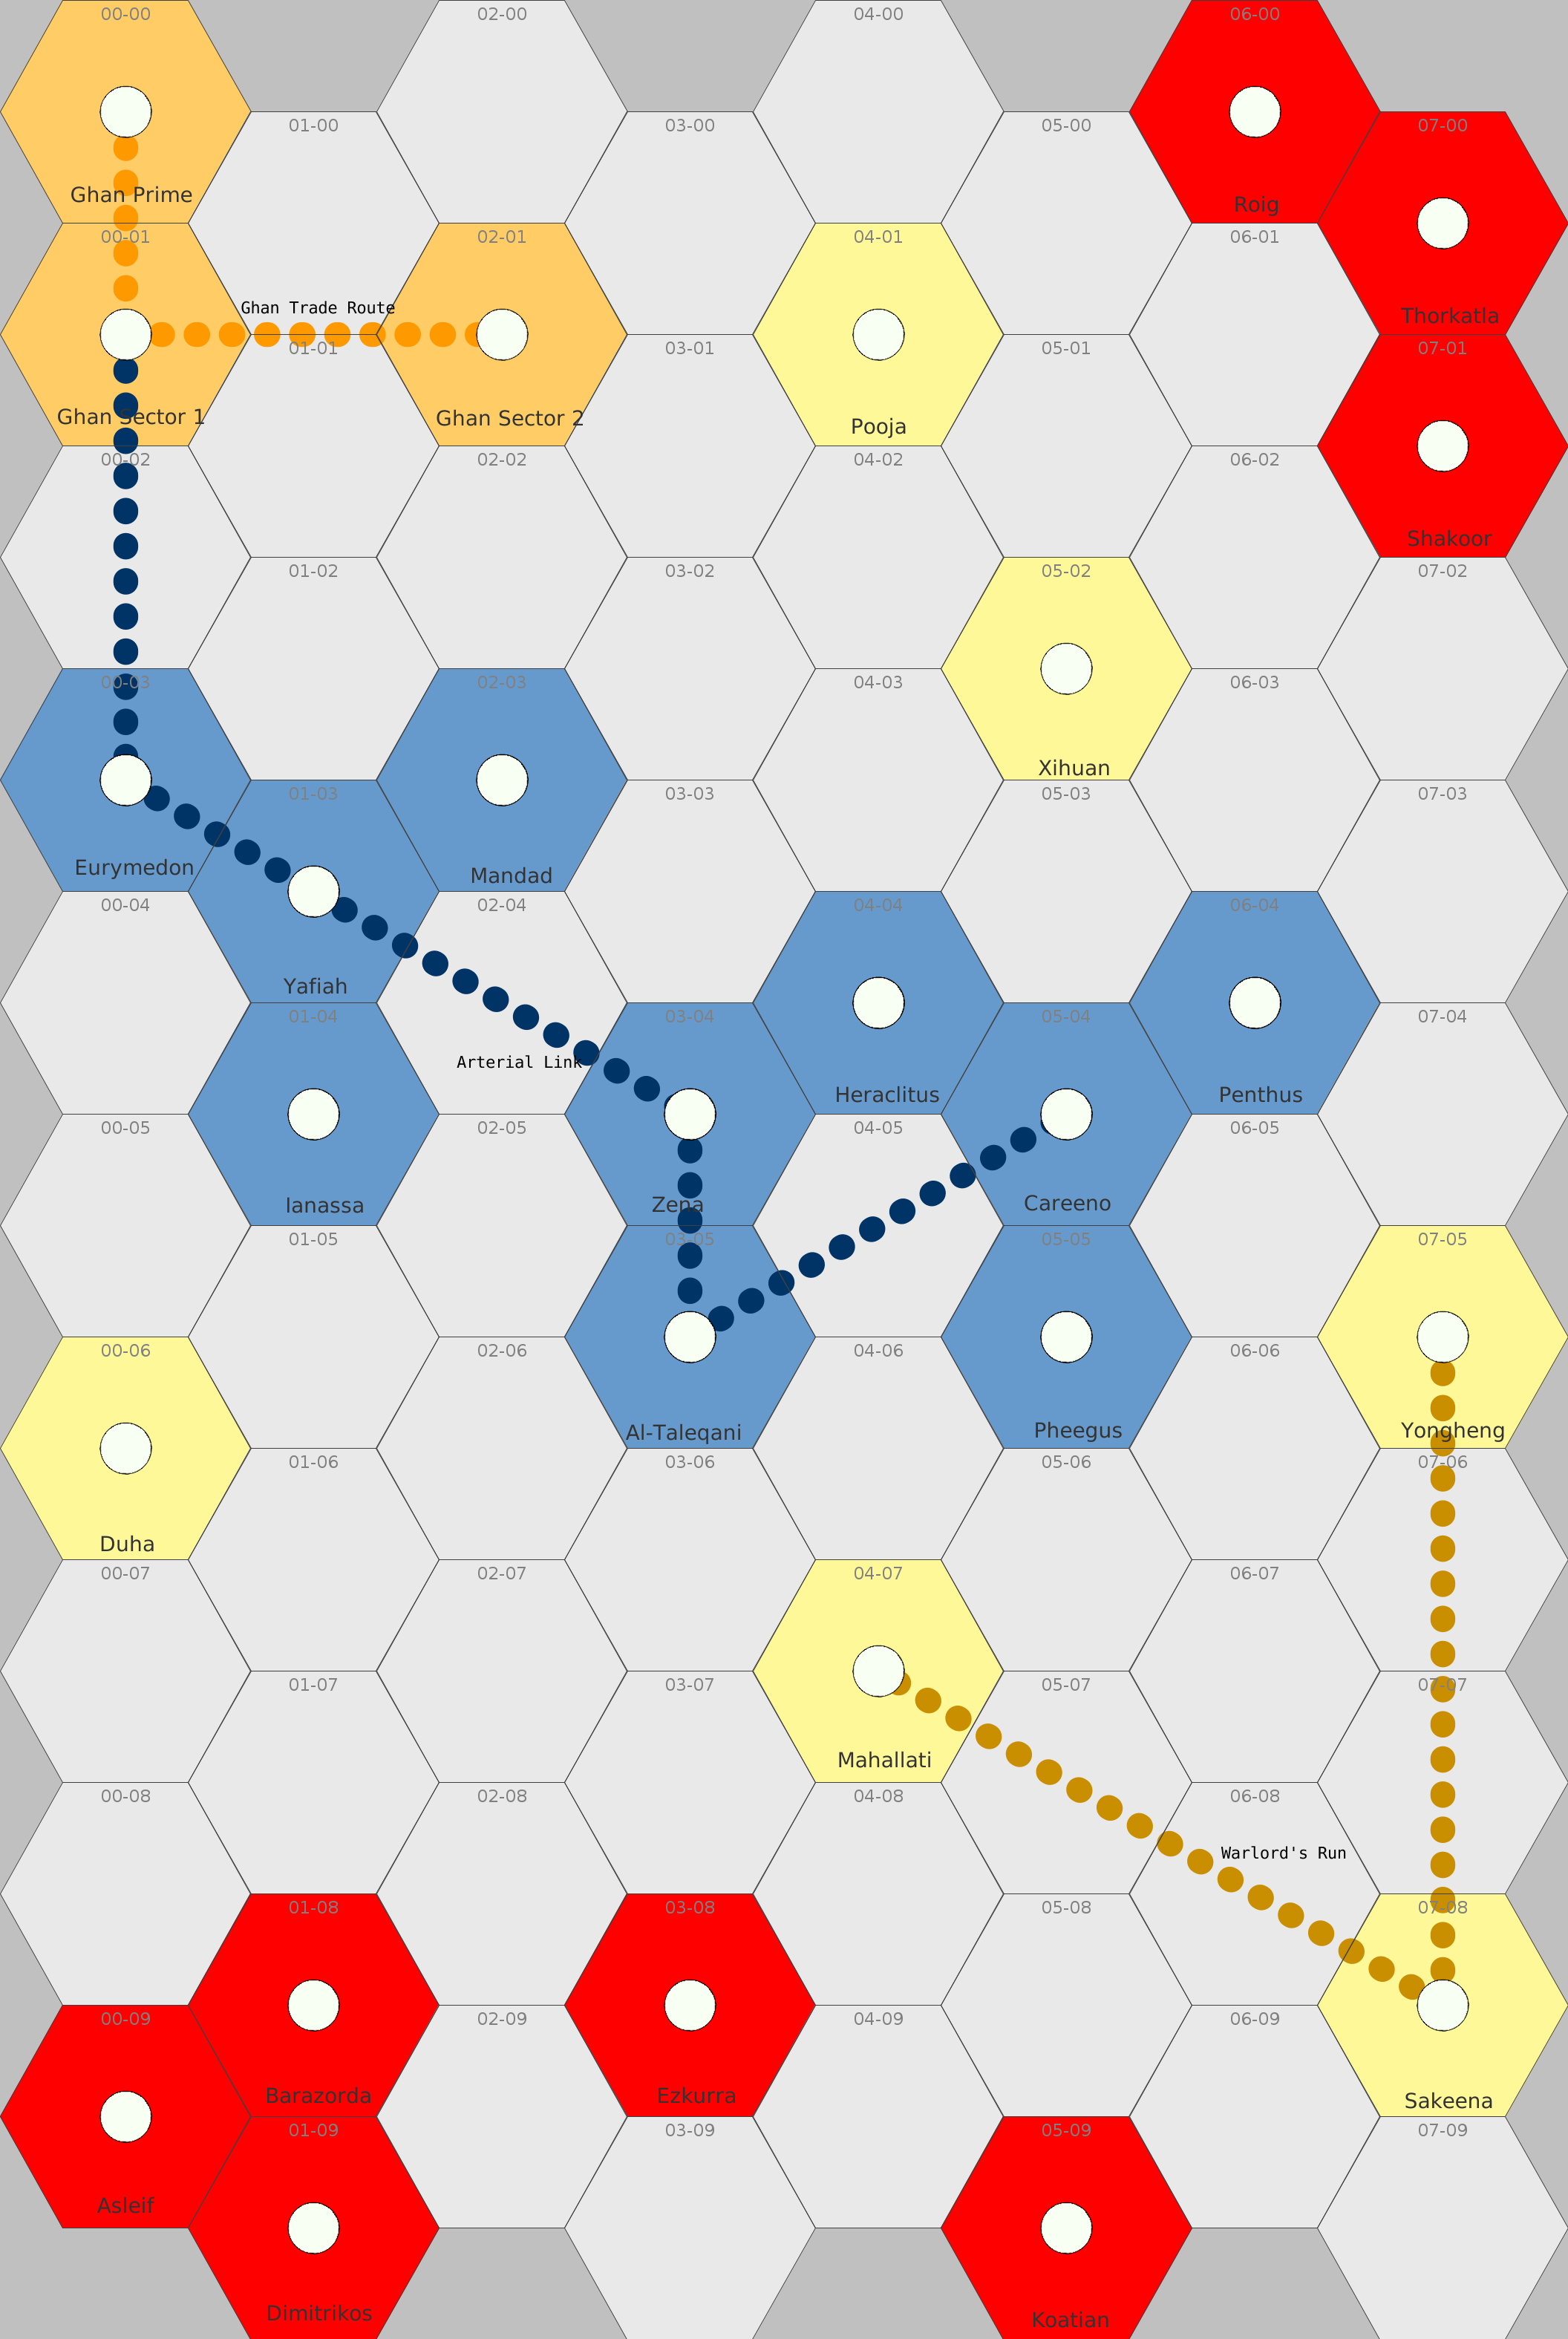
\includegraphics[height=220mm]{sectormap}
\end{center}

\newpage

\begin{multicols}{2}

  \subsection{Sector Overview}

  Sector Shangra Omega consists of 10 \textit{Core} systems (blue), 6 \textit{Independent} systems (yellow), 3 \textit{Ghan} systems (orange) and possibly up to 8 \textit{Lost} systems (red). The systems that surround Shangra Omega are largely unexplored, and Pre-Surge star charts are severely out of date. The sector map used by navigators today are the result of intrepid explorers braving the Black and re-charting the stars.
  
  \begin{redtable}{\linewidth}{bsb}
    \textbf{Name} & \textbf{System} & \textbf{Type}\\
    Al-Taleqani & 03-05 & Core\\
    Asleif & 00-09 & Lost\\
    Barazorda & 01-08 & Lost\\
    Careeno & 05-04 & Core\\
    Dimitrikos & 01-09 & Lost\\
    Duha & 00-06 & Independent\\
    Eurymedon & 00-03 & Core\\
    Ezkurra & 03-00 & Lost\\
    Ghan Prime & 00-00 & Ghan\\
    Ghan Sector 1 & 00-01 & Ghan\\
    Ghan Sector 2 & 02-01 & Ghan\\
    Heraclitus & 04-04 & Core\\
    Ianassa & 01-04 & Core\\
    Koatian & 05-09 & Lost\\
    Mahallati & 04-07 & Independent\\
    Mandad & 02-03 & Core\\
    Penthus & 06-04 & Core\\
    Pheegus & 05-05 & Core\\
    Pooja & 04-01 & Independent\\
    Roig & 06-00 & Lost\\
    Sakeena & 07-08 & Independent\\
    Shakoor & 07-01 & Lost\\
    Thorkatia & 07-00 & Lost\\
    Xihuan & 05-02 & Independent\\
    Yafiah & 01-03 & Core\\
    Yongheng & 07-05 & Independent\\
    Zena & 03-04 & Core\\
  \end{redtable}
  
  \subsection{Core Systems}

  \textbf{The Core} is the name given to the systems that make up the \textbf{United Planets}, a loose federation of star systems that share a common legal framework and similar military structures. Planets, Habitats, Space Stations and Star Systems are allowed to largely govern themselves, but are subject to Universal Decrees voted upon by the United Systems Council. Each star system that has a habitable planet sends 10 Delegates to the Council (regardless of the number of planets, colonies, space stations, or other habitation in that system), and Delegates do not necessarily need to be democratically appointed.
  
  \begin{genericsection}{Al-Taleqani}
  The most populous star system and a cultural force in the known Black. If you want to find something special, odds are that you can find it in Al-sahhah (the main planet, boasting a population of over 1 billion citizens). Despite it's arabic name, the sector is culturally diverse and boasts the largest population of Ay-Matak in the sector. Many across the Black make their way to Al-Taleqani in the hopes of striking it rich in the mines of Khadim, in a popular Al-Rhul Productions sim-sense experience, or in the hustle and bustle of the streets of Al-sahhah.
  
  The prominent idealogy of the system generally focuses on liberty, individual freedoms and the unity and growth of the United Planets.
  \end{genericsection}
  
  \begin{genericsection}{Careeno}
  Commonly known as the "\textit{Blue Collar System}", Careeno is largely known for it's primary industries. In the skies above Raghd are the large space craft manufactories, along the plains of Mahats are the farms that feed billions, and on Polypheme hums the factories that keep our economy going. As the second most populous system in the United Planets (and a industrial powerhouse), Careeno has enough political clout to challenge the powerful Al-Taleqani Delegates in the Council.
  
  The prominent idealogy of the system generally focuses on issues that affect the industrial and agricultural working class. This means that the populace strongly leans towards unions, universal healthcare and other forms of workplace protections.
  \end{genericsection}
  
  \begin{genericsection}{Eurymedon}
  Eurymedon is the most curious system in United Planets. On the one side is Aerope, known for it's fear of foriegners and outsiders. And on the other side is Olaria, known for being open to almost everyone and every idea. In between the two is Nishtha, an Olarian colony that is really only known for it's intact Pre-Surge ruins that serve as a pilgramage site for Pre-Surge enthusiasts. Despite the heated arguments and debates between Aerope and Olaria, war has never threatened the system.
  
  Idealogy largely depends on the planet. Aerope is largely isolationist, joining the United Planets reluctantly so that they could enjoy the protection and economy of the Federation (however the planetary government is rather lax in enforcing United Planet laws, especially those regarding psionics). Olaria (and Nishtha) embraces virtually everything.
  \end{genericsection}
  
  \begin{genericsection}{Heraclitus}
  Parezi is one of the few habitated airless planets in the Sector, and it is reknowned for it's bubble cities that sprawl across it's surface. The system itself is devoted to mining the mineral dense asteroid fields and gas giants. 
  
  Although the system was largely founded by Al-Taleqani entreprenuers, the working class find a lot in common with the citizens of Careeno. As such, the people are split in their loyalties to these two political powerhouses.
  \end{genericsection}
  
  \begin{genericsection}{Ianassa}
  Ianassa is known around the Black for it's partially intact Pre-Surge archive on Hildegunn. This has led to many Universities, Academies and corporate R\&D departments being established on the planet, devoted to unlocking the secrets of the past. The quarantined planet Androcles is also in the system, locked away because the unstable magnetosphere and severe weather patterns have marooned many space craft on it's barren surface. There are rumours that there is another Pre-Surge archive on Androcles, but that it contains dangerous knowledge that could destroy the Sector.
  
  The ideology of the system largely focuses on knowledge, education and academic merit.
  \end{genericsection}
  
  \begin{genericsection}{Mandad}
  The most heavily regulated and restricted system in the United Planets. Primitive sentient aliens were discovered on Aranzta, leading to the Arantza government to the policy of non-interference and dedicating large reserves for the primitives to inhabit. And on Merlo is one of the last remaining refuges for Psionic schools, and the only one to be found in the United Planets. Because of a latent fear of psionics and the possibility that they will bring about the Surge, Merlo is quarantined and it's Psionics heavily regulated.
  
  On Aranzta, the population see that their non-interference methods follow in the path of Pre-Surge civilisations and see themselves the traditional inheritors of the past. Merlo, on the other hand, wants dramatic government reforms when it comes to the issue of Psionics.
  \end{genericsection}
  
  \begin{genericsection}{Penthus}
  Pethus is the only Christian-ruled system in the sector. Bergthora clung to it's faith after the Surge, although it's teachings are different to classical Catholicism due to theological drift. An on-going problem with pirates from the Shakoor system led to the colonisation of Semera, a military output designed to ward off undesirables.
  
  The ideology of the system largely revolves around conservatism, religious ideas and traditional values.
  \end{genericsection}
  
  \begin{genericsection}{Pheegus}
  Pheegus is usually seen as a tourist destination for the citizens of the United Systesm. Ballesteros is an ocean planet that boasts huge floating cities filled with assorted activities for visitors to do. It also strictly maintains it's Pre-Surge sea-faring culture in an effort to preserve it's past, although some cynics see the cultural shows and festivals as another way to fleece credits from tourists. Orithyia is also a tourist destination but because it boasts the largest population of Altered Humans. Orithyia is known across the Black for it's "Freak shows".
  \end{genericsection}
  
  \begin{genericsection}{Yafiah}
  A common saying across the Black is "\textit{All Bank Accounts leads to Mecisteus}". The sole planet of the Yafiah system has built a reputation as a financial powerhouse. This is mainly due to it's strong protection and privacy laws, which allows corporations and individuals to safely and securely horde their credits.
  \end{genericsection}
  
  \begin{genericsection}{Zena}
  While Al-Taleqani and Careeno are the superpowers of interstellar politics, Zena is the close third. It's position in the middle of the United Systems' territory has meant that it has become the undisputed Trade Hub. It boasts respectable spaceyards in orbit above Marider, while Thurid is known for it's industrial output and trading stations.
  
  It's ideology is varied as the population values it's role as the "arbiter" of interstellar politics, often becoming the deciding vote between the Al-Taleqani and Careeno blocs.
  \end{genericsection}
  
  \subsection{Independent Systems}

  Independent systems are those that choose to remain seperate from the United Systems. Some chose not to join because they feel that the strict 10 Delegates per system would unfairly discriminate their large populations. Others stay away because the Decrees do not align with their local laws and customs. And some wish to remain as black market havens. Whatever the reason, Independent systems are considered the "Wild West" of the Black.
  
  \begin{genericsection}{Sakeena}
  Sakeena is a largely self-sufficient star system that strictly follows a protectionist foriegn policy. They see the United Systems as a threat to their sovereignity, and actively work to make sure the United Systems do not interfere with their 'sphere of influence'. Many think that the Sakeena system actively encourages the tensions within the Mahallati and Yongheng systems so that they cannot join the United Systems.
  \end{genericsection}
  
  \begin{genericsection}{Yongheng}
  The planet Vargos in the Yongheng system is embroiled in a decades long civil war. The war originally broke out after the planet Theano was colonised, with six factions claiming ownership. The six factions are: Associated States of Yongheng, Federated States of New Shanghai, South Sodality, Theano Pact, Union of Vargos, and the Vargos Commonality. Vargos itself has been spared the ravages of war as most fighting is done on the surface of Theano, with each faction fighting over patches of territory on the planets surface.
  \end{genericsection}

  \subsection{Ghan Systems}
  
  Ghan systems are, quite simply, the home systems for the Ghantak. Ghan Prime has the homeworld of Ghan, and the Ghantak were able to colonise (at least) two other star systems before the Surge. These systems have all managed to survive the Surge and re-establish contact with each other, but choose to remain seperate from the United Systems. They are led by an Empress who resides in Ghan Prime, but each planet is governed by a Hive Queen that has the freedom to do as she pleases.

  \subsection{Lost Systems}
  
  Lost systems are those that are speculated to still exist, but no formal communication or expedition exist to explore them fully. Travel to the Lost systems are fraught with danger, as many do not return.

  \subsection{Tech-Levels}
  \label{sec:sector-tech-levels}

  Tech-Levels are a standard way to catergorise the differing manufacturing capabilities of a planet. Some worlds are purposely kept at low tech-levels as they provide primary trade resources for high tech-level worlds (such as agriculture).
  
  To see how Gear and Tech-Levels relate to each other, please refer to the \textit{\hyperref[sec:gear-rules]{Gear Tech-Level section}}

  \begin{standardtable}{\linewidth}{ssb}
    \textbf{Level} & \textbf{Description} & \textbf{Example}\\
    0 & Stone & Stone, human power\\
    1 & Ancient & Metals, domestic animals, steam engine\\
    2 & Industrial & Fossil fuels, factories, simple machines\\
    3 & Mechanized & Computers, satellites, 20th century era tech\\
    4 & Interstellar & IDD, energy weapons, cyberware \\
    5 & Advanced & Specialized knowledge in a technological field\\
    6 & Pre-Surge & Psionic tech, TDD, exotic tech\\
  \end{standardtable}

  % ATB Rating
  \subsubsection{ATB classification}
\label{sec:sector-atb}

The \textbf{Atmospheric - Temperature - Biosphere} (ATB) rating is the standard classification system for worlds, planets and other naturally occuring stellar bodies. An ATB gives a general overview about the suitability for habitation, or at the very least an idea of what risks there are in colonising the world. The classification uses 3 letters, one for each of the categories of Atmosphere, Temperature and Biosphere.

\subsubsection{Atmosphere}

\begin{genericsection}{A (Airless)}
  There is little to no atmosphere to speak of. Requires a space suit with a constant supply of oxygen
\end{genericsection}

\begin{genericsection}{B (Breatheable)}
  A mix of gases that is within the breatheable range for organic beings. Since each planet has different mixtures, foriegners are always aware of a "new world stink"
\end{genericsection}

\begin{genericsection}{C (Corrosive)}
  Dangerously hostile atmosphere, even with conventional suits and other protective gear. The atmosphere is extremely toxic, and actively corrodes non-native materials
\end{genericsection}

\begin{genericsection}{G (Inert Gas)}
  Atmosphere consists of gases that are not breatheable by organic beings. The atmosphere is otherwise not hostile or poisonous, but requires a constant source of oxygen
\end{genericsection}

\begin{genericsection}{T (Thick)}
  The atmosphere contains gases that are heavier and thicker than an organic can handle. Organics will require the aid of a filtration mask to breathe the atmosphere. It is considered toxic if an organic decides to breathe the air straight over long periods of time (organics can breathe the air for short periods of time, although their breathing will be laboured)
\end{genericsection}

\begin{genericsection}{X (Toxic)}
  These worlds are much more aggressively hostile than corrosive (C) worlds. These worlds have toxic molecules that are able to bypass suit seals during the corrosion process, meaning that they must be purified at regular intervals, reducing the oxygen supply substantially
\end{genericsection}

\subsubsection{Temperature}

\begin{genericsection}{F (Frozen)}
  Average temperature that is close to absolute zero. Some are so cold that the gases have solidified
\end{genericsection}

\begin{genericsection}{C (Cold)}
  These worlds are uncomfortably cold, but are survivable with suitable heavy clothing
\end{genericsection}

\begin{genericsection}{T (Temperate)}
  These worlds have temperature ranges that are similar to Earth
\end{genericsection}

\begin{genericsection}{W (Warm)}
  These worlds are uncomfortably warm, but are survivable. They are either desert worlds, or have thick, humid jungles
\end{genericsection}

\begin{genericsection}{B (Burning)}
  Average temperatures that is close to boiling. Some are so hot that metals exist in molten form
\end{genericsection}

\begin{genericsection}{V (Varied)}
  These worlds have a wide range of temperatures, either due to unique geological features or varying orbits around their star
\end{genericsection}

\subsubsection{Biosphere}

\begin{genericsection}{R (Remnants)}
  The wreckage and ruins of a dead ecology
\end{genericsection}

\begin{genericsection}{M (Microbial)}
  Non-sentient micro-organisms that can exist in almost all types of environments (such as slimes, bacteria, fungus). They may or may not be dangerous
\end{genericsection}

\begin{genericsection}{Z (None)}
  For some reason or other, life did not evolve on this world
\end{genericsection}

\begin{genericsection}{C (Compatible)}
  Substantial portion of native life is biologically compatible with human nutritional needs
\end{genericsection}

\begin{genericsection}{I (Incompatible)}
  None of the native life is biologically compatible with human nutritional needs. Microbial life could potentially be highly allergenic to humans
\end{genericsection}

\begin{genericsection}{H (Hybrid)}
  The native flora and fauna have been intermixed with imported species from Earth. They may or may not be compatible, but are not otherwise hostile
\end{genericsection}

\begin{genericsection}{E (Engineered)}
  Are either paradise planets that have been carefully sculpted, or living forges that produce foodstuffs and minerals for trade
\end{genericsection}

  % Military
  \subsection{Military Ranks}

There will always be a need for a standing military service, and in the Pre-Surge days the powers that be decided on a single rank system for all servicemen (whether army or navy). This standard has been carried on after the Surge, and even warring factions on Independant worlds are known to use the system.

\subsubsection{Enlisted}

Enlisted men provide the manpower for the military services. They serve as the marines, infantry, pilots, engineers, and any other role that is required of them. They can advanced through the ranks in either leadership roles or as specialised experts in their field.

\begin{standardtable}{\linewidth}{sb}
  \textbf{Rank} & \textbf{Duties} \\
  Private (PVT) & The lowest rank\\
  Specialist (SPC) & Used to designate an individual with special skills\\
  Corporal (CPL) & Leader of a team (4 servicemen), or Senior specialists or administrative staff\\
  Sergeant (SGT) & Leader of a section (2-3 teams, 8-15 servicemen), or Senior staff for command-level officers\\
  Master Sergeant (MSG) & Highest rank for non-commissioned officers. Senior staff or supervisors of the enlisted men\\
\end{standardtable}

\subsubsection{Officers}

Officers provide leadership for the men under their command. They command large numbers of men or military spacecraft, and only rise up the ranks through exemplary service.

\begin{standardtable}{\linewidth}{sb}
  \textbf{Rank} & \textbf{Duties} \\
  Ensign (ENS) & Entry-level rank for officers. Generally put in charge of a secion with the aide of a Sergeant\\
  Lietenant (LT) & Leader of a platoon (2-3 sections, 16-45 servicemen), or subordinate for command-level officers\\
  Major (MAJ) & Leader of a company (3-4 platoons, 50-180 servicemen), or commands a small spacecraft\\
  Commander (CDR) & Leader of a battalion (3-4 companies, 200-700), or commands a medium spacecraft\\
  Captain (CPT) & Leader of a brigade (3-4 battalions, 1000-3000), or commands a large spacecraft\\
  Colonel (COL) & Leader of a division (4-5 brigades, 4000-15000), or commands a flotilla (2+ spacecraft)\\
  Vice Admiral (VADM) & Leader of a corps (2-3 divisions, 15000-45000), or commands a group (2+ flotilla). Some infantry forces prefer the older "Lietenant General"\\
  Admiral (ADM) & Leader of an army (2-3 corps, 80000+), or commands a fleet (2+ groups). Some infantry forces prefer the older "General". Seniority is designated by stars, with the highest achievable rank is a 6-star Admiral/General\\
\end{standardtable}

\end{multicols}

\newpage

% Worlds
% =================
% Worlds
% =================
\subsection{Worlds}

  \subsubsection{Core Worlds}

  \begin{powertable}{ p{.10\textwidth} p{.10\textwidth} p{.05\textwidth} p{.05\textwidth} p{.20\textwidth} p{.35\textwidth} }
    \textbf{Name} & \textbf{A-T-B} & \textbf{Pop.} & \textbf{TL} & \textbf{Sector} & \textbf{Tags}\\
    Aerope	    & T-C-H &	10M+  & 3	& Eurymedon (00-03)   & Bigotry, Fear of Psionics\\
    Al-sahhah   & B-V-C & 1B+   & 4 & Al-Taleqani (03-05) & Specialised Technology, Regional Hegemon\\
    Androcles   & B-T-R & 100K+ & 3 & Ianassa (01-04)     & Freak Geology, Quarantined\\
    Arantza     & T-W-C & 1M+   & 4 & Mandad (02-03)      & Restrictive Laws, Primitive Aliens\\
    Ballesteros & T-T-C & 1M+   & 4 & Pheegus (05-05)     & Rigid Culture, Seagoing cities\\
    Bergthora   & A-T-M & 1M+   & 5 & Penthus (06-04)     & Heavy Industry, Theocracy\\
    Hildegunn   & B-W-C &	100K+	& 4	& Ianassa (01-04)     & Pre-Surge Archive, Intelligence\\
    Khadim	    & T-C-I & 100K+ & 3	& Al-Taleqani (03-05) & Gold Rush, Colonised\\
    Mahats	    & T-T-E &	100K+ &	4 & Careeno (05-04)     & Agriculture, Theocracy\\
    Marider	    & A-T-R & 10M+	& 5	& Zena (03-04)        & Heavy Mining, Major Spaceyard\\
    Mecisteus   & B-T-C & 100M+ & 4 & Yafiah (01-03)      & Banking, Local Specialiaty\\
    Merlo       & B-T-I & 1M+   & 3 & Mandad (02-03)      & Psionic School, Quarantined\\
    Nishtha     &	B-C-C &	100K+	& 4	& Eurymedon (00-03)   & Pre-Surge Ruins, Pilgrimage\\
    Olaria      & G-T-C & 10M+  & 5 & Eurymedon (00-03)   & Pre-Surge Cultists, Xenophiles\\
    Orithyia    & G-T-E &	100K+	& 4	& Pheegus (05-05)     & Altered Humans, Agriculture\\
    Parezi	    & A-W-M & 1M+	  & 4	& Heraclitus (04-04)  & Heavy Mining, Bubble Cities\\
    Polypheme	  & G-V-I & 10M+  &	4 & Careeno (05-04)     &	Trade Hub, Specialised AI\\
    Raghd       & B-T-Z & 1B+   & 5 & Carreno (05-04)     & Flying Cities, Major Spaceyard\\
    Semera      & B-V-I &	100K+	& 4	& Penthus (06-04)     & Outpost, Police State\\
    Thurid      & B-C-C & 100M+ & 4	& Zena (03-04)        & Trade Hub, Heavy Industry\\
  \end{powertable}
 
  \subsubsection{Independent Worlds}

  \begin{powertable}{ p{.10\textwidth} p{.10\textwidth} p{.05\textwidth} p{.05\textwidth} p{.20\textwidth} p{.35\textwidth} }
    \textbf{Name} & \textbf{A-T-B} & \textbf{Pop.} & \textbf{TL} & \textbf{Sector} & \textbf{Tags}\\
    Amir        & B-T-C & 1M+   & 4 & Duha (00-06)      & Oceanic World, Fear of Psionics\\
    Ba'albaki	  & B-C-H &	1M+   &	4	& Xihuan (05-02)    & Psionic School, Psionic Worship\\
    Dirce       & B-V-C & 100K+ & 4 & Pooja (04-01)     & Desert World, Civil War\\
    Garrastazu  & T-T-H & 1M+   & 3 & Duha (00-06)      & Violent Sectarians, Heavy Mining\\
    Georghiou	  & B-T-E & 1M+   &	3 &	Sakeena (07-08)   & Colonised, Agriculture\\
    Oeneus      & G-T-I & 1M+   & 3 & Sakeena (07-08)	  & Colonised, Heavy Industry\\
    Sakeena     & T-T-I & 10B+  & 5 & Sakeena (07-08)   & Major Spaceyard, Police State\\
    Salimah	    & B-T-E & 100K+ &	4	& Mahallati (04-07) & Rigid Culture, Eugenic Cultists\\
    Theano      & B-F-H & 100K+ & 3 & Yongheng (07-05)  & Outpost, Hatred\\
    Thorhalla   & T-V-H & 10M+  & 4 & Xihuan (05-02)    & Tyranny, Bigotry\\
    Vinata      & G-W-C & 1M+   & 4 & Mahallati (04-07) & Civil War, Bubble Cities\\
    Vargos      & T-T-H & 1B+   & 3 & Yongheng (07-05)  & Cold War, Warlords\\
  \end{powertable}

  \subsubsection{Lost Worlds}

  \begin{powertable}{ p{.10\textwidth} p{.10\textwidth} p{.05\textwidth} p{.05\textwidth} p{.20\textwidth} p{.35\textwidth} }
    \textbf{Name} & \textbf{A-T-B} & \textbf{Pop.} & \textbf{TL} & \textbf{Sector} & \textbf{Tags}\\
    Akriti      & A-T-C & ?     & ? & Koatian (05-09)     & Zombies, Out of Contact\\
    Chloe       & B-T-C & 100K+ & 2 & Ezkurra (03-08)     & Minimal Contact, Fear of Tech\\
    Echepolos   & ?-T-M & ?     & ? & Shakoor (07-01)     & Radioactive, Tomb World\\
    Gyda        & B-C-C & 10K+  & 3 & Aslief (00-09)      & Xenophobes, Pre-Surge Archive\\
    Maqsood     & B-C-H & 100K+ & 3 & Dimitrikos (01-09)  & Psionic Worship, Out of Contact\\
    Purva       & B-F-C & 100K+ & 3 & Barazorda (01-08)   & Feral, Pre-Surge Cultists\\
    Pylaimenos  &	A-V-Z & ?     &	? & Thorkatia (07-00)   &	Sealed Menace, Unbreaked AI\\
    Sagari      & B-T-C & 10K+  & 4 & Shakoor (07-01)     & Hostile Space, Badlands World\\
    Xanthippe	  & B-T-H &	1M+   &	4	& Roig (06-00)        & Tyranny, Theocracy\\
  \end{powertable}

  \subsubsection{Ghan Worlds}

  \begin{powertable}{ p{.10\textwidth} p{.10\textwidth} p{.05\textwidth} p{.05\textwidth} p{.20\textwidth} p{.35\textwidth} }
    \textbf{Name} & \textbf{A-T-B} & \textbf{Pop.} & \textbf{TL} & \textbf{Sector} & \textbf{Tags}\\
    Ghalla	& B-W-C &	100K+	& 4	& Ghan Sector 1 (00-01) & Trade Hub, Local Speciality\\
    Ghan    & B-T-C & 10B+  & 5 & Ghan (00-00)          & Banking, Regional Hegemon\\
    Ghatla	& T-W-C &	100K+	& 4	& Ghan (00-00)          & Freak Weather, Agriculture\\
    Gharda  &	B-W-C & 100K+ &	4	& Ghan Sector 2 (02-01) & Oceanic, Major Spaceyard\\
    Ghusha	& A-C-M	& 100K+ &	4	& Ghan Sector 2 (02-01) & Heavy Mining, Freak Geology\\
  \end{powertable}

% Business groups and factions
% =================
% BUSINESS GROUPS AND FACTIONS
% =================
\subsection{Corporations}
  
  \subsubsection{Core Corporations}

  \begin{powertable}{ p{.20\textwidth} p{.35\textwidth} p{.35\textwidth} }
    \textbf{Business} & \textbf{Name} & \textbf{Headquarters}\\
    Agriculture   & Tatum Farming Collective  & Arantza, Mandad (02-03)\\
    Agriculture   & Aqualis Food Conglomerate & Mahats, Careeno (05-04)\\
    Agriculture   & SuriTech Foodstuffs       & Orithyia, Pheegus (05-05)\\
    Astronautics  & Mavridou Cooperative      & Raghd, Careeno (05-04)\\
    Astronautics  & Quebe-Luxfause Systems    & Marider, Zena (03-04)\\
    Biotech       & Interstellar Genetics Inc & Mahats, Careeno (05-04)\\
    Biotech       & Morgath Industries        & Khadim, Al-Taleqani (03-05)\\
    Biotech       & Umbrella Coorporation     & Ballestreros, Pheegus (05-05)\\
    Construction  & Novaplex                  & Mecisteus, Yafiah (01-03)\\
    Construction  & Panstellar Zaibatsu       & Bergthora, Penthus (06-04)\\
    Cybernetics   & Imaharatronics            & Olaria, Eurymedon (00-03)\\
    Cybernetics   & Lacuna, Inc.              & Hildegunn, Ianassa (01-04)\\
    Cybernetics   & Wayne Enterprises         & Thurid, Zena (03-04)\\
    Electronics   & Altin Alliance            &	Polypheme, Careeno (05-04)\\
    Electronics   & Gowix Computers           & Hildegunn, Ianassa (01-04)\\
    Electronics   & MicroData Technologies    & Al-sahhah, Al-Taleqani (03-05)\\
    Entertainment & Al-Rhul Productions       &	Al-sahhah, Al-Taleqani (03-05)\\
    Entertainment & Haen Multistellar         & Olaria, Eurymedon (00-03)\\
    Exploration   & Bellixan Endeavors        & Khadim, Al-Taleqani (03-05)\\
    Exploration   & Degan Explorations        & Nishtha, Eurymedon (00-03)\\
    Finance       & Anistonopoulos Clan       & Mecisteus, Yafiah (01-03)\\
    Finance       & Gringotts                 & Mecisteus, Yafiah (01-03)\\
    Fishing       & Nopoulos Partnership      & Ballesteros, Pheegus (05-05)\\
    Fuel Refinery & Burns Industries          & Raghd, Careeno (05-04)\\
    Fuel Refinery & Parezi Energy             & Parezi, Heraclitus (04-04)\\
    Genetics      & Gentik                    & Bergthora, Penthus (06-04)\\
    Genetics      & Orithyia Genetics         & Orithyia, Pheegus (05-05)\\
    Genetics      & Nazari Cooperative        & Olaria, Eurymedon (00-03)\\
    Manufacturing & Gorallis Metalworking     & Raghd, Careeno (05-04)\\
    Manufacturing & Kroeskin Fabrications     & Thurid, Zena (03-04)\\
    Manufacturing & Merr-Sonn Industrial      & Al-sahhah, Al-Taleqani (03-05)\\
    Mining        & Colonial Mining           & Parezi, Heraclitus (04-04)\\
    Mining        & Nexcore Mining Corp       & Marider, Zena (03-04)\\
    Pharma.       & Saraphis Megacorp         & Mecisteus, Yafiah (01-03)\\
    Pharma.       & Velunza Circle            & Olaria, Eurymedon (00-03)\\
    Programming   & HoloGraphics Interstellar & Mecisteus, Yafiah (01-03)\\
    Programming   & Perzome SoftWEAR          & Olaria, Eurymedon (00-03)\\
    Programming   & Pied Piper                & Hildegunn, Ianassa (01-04)\\
    Robotics      & Advanced Ideas Mechanics  & Marider, Zena (03-04)\\
    Robotics      & Aperture Science, Inc.    & Thurid, Zena (03-04)\\
    Robotics      & Cyberdyne Systems         & Bergthora, Penthus (06-04)\\
    Security      & Asset Group Solutions     & Al-sahhah, Al-Taleqani (03-05)\\
    Security      & Barichello Multistellar   & Semera, Penthus (06-04)\\
    Security      & Santhe Security           & Mecisteus, Yafiah (01-03)\\
    Spacecraft    & Curich Engineering        & Marider, Zena (03-04)\\
    Spacecraft    & Ferris Spacecraft         & Marider, Zena (03-04)\\
    Spacecraft    & Solar Spacecraft          & Raghd, Careeno (05-04)\\
    Spacecraft    & Starlette Industries      & Raghd, Careeno (05-04)\\
    Snacks        & Buy n Large               & Thurid, Zena (03-04)\\
    Snacks        & Los Pollos Hermanos       & Al-sahhah, Al-Taleqani (03-05)\\
    Weapons       & Al-Astra Association      & Al-sahhah, Al-Taleqani (03-05)\\
    Weapons       & Stark Industries          & Thurid, Zena (03-04)\\
  \end{powertable}
  
  \subsubsection{Independant Coorporations}
  
  \begin{powertable}{ p{.25\textwidth} p{.35\textwidth} p{.35\textwidth} }
    \textbf{Business} & \textbf{Name} & \textbf{Headquarters}\\
    Fishing       & Faraj Fishing             & Amir, Duha (00-06)\\
    Illicit Drugs & Zea Outfit	              & Vinata, Mahallati (04-07)\\
    Illicit Drugs & Spiker Group              & Dirce, Pooja (04-01)\\
    Piracy        & Magnus Syndicate          & Sagari, Shakoor (07-01)\\
    Spacecraft    & Ghan Spacecraft           & Gharda, Ghan Sector 2 (02-01)\\
    Spacecraft    & Sakeena Shipyards         & Sakeena, Sakeena (07-08)\\
    Weapons       & Cafu Pact                 & Dirce, Pooja (04-01)\\
    Weapons       & Jayhoon Faction           & Vinata, Mahallati (04-07)\\
    Weapons       & Striker Ring              & Sagari, Shakoor (07-01)\\
    Weapons       & West Wind Outfit          & Vargos, Yongheng (07-05)\\
    Xenotech      & Ghan Systems              & Ghalla, Ghan Sector 1 (00-01)\\
  \end{powertable}

% Political groups and factions
% =================
% POLITICAL GROUPS AND FACTIONS
% =================
\subsection{Politics}
  
\subsubsection{United Planet Factions}

\begin{redpowertable}{ p{.20\textwidth} p{.05\textwidth} p{.25\textwidth} p{.4\textwidth} }
  \textbf{Name} & \textbf{Seats} & \textbf{Homeworld} & \textbf{Issues}\\
  Buffalo Party     & 5   & Arantza, Mandad (02-03)         & Culture, Traditionalists, Free Market \\
  Cerulean Guild    & 2   & Mecisteus, Yafiah (01-03)       & Progressives, Government reform, Industrial reform, Free Market\\
  Cobalt Consensus  & 7   & Raghd, Careeno (05-04)          & Industrialists, Welfare, Xenophiles \\
  Democratic Party	& 13  & Thurid, Zena (03-04)            &	Government reform, Foreign Policy, Xenophiles\\
  Freedom Element	  & 1   & Mecisteus, Yafiah (01-03)       &	Elitists, Foreign Policy, Protectionist, Autarky (Self-sufficiency), Xenophobia\\
  Homeland Alliance	& 3   & Ballesteros, Pheegus (05-05)    & Bigotry, Culture, Traditionalists, Protectionists\\
  Iron Front	      & 11  & Parezi, Heraclitus (04-04)      &	Working Class, Protectionist, Poverty, Welfare\\
  Libertarian       & 5   & Mecisteus, Yafiah (01-03)       & Progressive, Individual Rights, Industrial reform, Free Market, Xenophiles\\
  Liberty Combine	  & 15  & Al-sahhah, Al-Taleqani (03-05)  &	Foreign Policy, Free Market, Individual Rights\\
  Fellowship        & 3   & Hildegunn, Ianassa (01-04)      &	Progressives, Socialists, Foriegn Policy, Individual Rights\\
  Popular Banner    & 5   & Aerope, Eurymedon (00-03)       &	Working Class, Bigotry, Immigration, Autarky (self-sufficiency)\\
  Psionic Union	    & 3   & Merlo, Mandad (02-03)           &	Psionics, Communists, Government Reform, Individual Rights\\
  Social Federation & 6   & Raghd, Careeno (05-04) 	        & Culture, Industry\\
  Tyrian Consensus	& 4   &	Bergthora, Penthus (05-04)      & Religion, Tradition\\
  Unified Planets   & 11  & Al-sahhah, Al-Taleqani (03-05)  &	Foriegn Policy, Military\\
  Victory Sodality	& 6   & Semera, Penthus (05-04)         &	Traditionalists, State Industry, Military\\
\end{redpowertable}

\begin{multicols}{2}

\subsubsection{Organised Religions}

\begin{genericsection}{Earth Standard}
Earth Standard is a loose classification for any religious system that can trace it's roots back to Earth. Religious belief is one of the few things people hang on to when trying to survive, and many stubbornly refuse to change. These religious beliefs are usually passed down from close family members or friends. Religions include Buddhism, Christianity, Hinduism, Islam, Jews, and Mormonism.
\end{genericsection}

\begin{genericsection}{Neofundamentalist Ideologists}
\textbf{No universal leadership}\\
Born in the classical philosphical teachings of Earth (especially Stoicism). NFI adherants believe in accepting your lot in life, actively resisting temptation, and using Science to further our understanding of the world
\end{genericsection}

\begin{genericsection}{New Catholics}
\textbf{Ruling Council on Bergthora, Penthus}\\
Cut off from the Vatican (and Earth), the primarily Catholic colony at Bergthora created their own Council of Cardinals to provide leadership for their faithful. The Council gradually took over the governance of the entire system. New Catholics are the largest Christian organisation in the sector, mainly because they accept differing ideas on the nature of God and were able to adopt practices of other Christians
\end{genericsection}

\begin{genericsection}{Quietist Muslims}
\textbf{Communal Democracy}\\
Largely concentrated on Mahats in the Careeno system. After the turbulent 21st Century, the Islamic faith began to reject the old power structures and began to democratically guide their faith in the best interests of the community. The faith largely shuns foriegn policy issues that do not affect their world, and strives to limit their involvement with the affairs of nonbelievers. They prefer to keep to their own kind and avoid positions of wealth and power
\end{genericsection}

\begin{genericsection}{Stellarist Muslims}
\textbf{Communal Democracy}\\
Largely concentrated on Mahats in the Careeno system. A reaction to the Quietist movement, Stellarists believe that the movement has drifted too far from the original teachings. Stellarists desire to reintegrate the Islam faith within the larger interstellar community, and allow their members to actively seek positions of power and wealth
\end{genericsection}

\begin{genericsection}{Syncretism}
\textbf{No universal leadership}\\
After the Surge, many colonies began to focus on survival instead of religious fundamentals. This has resulted in many planets mixing and matching tenets from a wide spectrum of beliefs. This is the most common religion found within the sector
\end{genericsection}

\end{multicols}

